% !TeX root = ..\protokoll.tex
\documentclass[../protokoll.tex]{subfiles}
\graphicspath{{\subfix{../images/}}}
\begin{document}
\part{Theorie}
Die elementaren Wissenselemente für die kommenden Versuche sollten aus der
Schule noch bekannt sein, jedoch werden diese hier nochmal kurz zusammengefasst.
Hierbei wird es um die Entstehung der verschiedenen Typen von Radioaktivität
gehen und um die beiden angewendeten Messmethoden 
(\textsc{Geiger-Müller-Zähler} und Szintillationsdetektor).

\section{Bezeichnungsweisen}
Um den nachfolgenden Abschnitt über die Schreibweise der Nukliden verstehen zu 
können, werden die folgenden Schreibweisen/Bezeichnungen engeführt:

\begin{table}[H]
    \caption{Benutzte Schreibweisen/Bezeichnungen in diesem Protokoll, entnommen aus \cite[S. 30]{script}}
    \centering
    \renewcommand{\arraystretch}{1.2}
    \begin{tabular}{|l|l|l|}
        \hline
        \textbf{Symbol} & \textbf{Einheit} & \textbf{Physikalische Größe} \\ \hline \hline
        $Z$ & & Ordnungs- oder Kernladungszahl: Zahl der Protonen im Atomkern \\ \hline
        $N$ & & Zahl der Neutronen in einem Atomkern \\ \hline
        $A = Z + N$ & & Massenzahl \\ \hline
        $p$ & & Proton \\ \hline
        $n$ & & Neutron \\ \hline
        $\beta^-$ & & Elektron \\ \hline
        $\beta^+$ & & Positron \\ \hline
        $\alpha$ & & Alpha-Teilchen \\ \hline
        $v$ & & Neutrino \\ \hline
        $\mathbf{\bar{v}}$ & & Antineutrino \\ \hline
        $\gamma$ & & Gammaquant \\ \hline
        $h$ & \unit{\joule\second} & Plancksche Konstante: $h = \qty{6.62606957(29)e-34}{\joule\second}$ \\ \hline
        $f$ & \unit{\per\second} & Frequenz eines Gammaquants \\ \hline
        $E=hf$ & \unit{\joule}, \unit{\electronvolt} & Energie eines Gammaquants;$ \qty{1}{\electronvolt} \approx \qty{1.602e-19}{\joule}$ \\ \hline
        $T_{1/2}$ & \unit{\second} & Halbwertszeit \\ \hline
        $\lambda = \ln \frac{2}{T_{1/2}}$ & \unit{\per\second} & Zerfallskonstante \\ \hline
        $\tau = \frac{1}{\lambda}$ & \unit{\second} & mittlere Lebensdauer \\ \hline
        $\mu_{\tau}$ & \unit{\per\cm} & Linearer Abschwächungskoeffizient für den Photoeffekt \\ \hline
        $\mu_{\sigma}$ & \unit{\per\cm} & Linearer Abschwächungskoeffizient für den \textsc{Compton}-Effekt \\ \hline
        $\mu_{\kappa}$ & \unit{\per\cm} & Linearer Abschwächungskoeffizient für die Paarerzeugung \\ \hline
        $\mu = \mu_{\tau} + \mu_{\sigma} + \mu_{\kappa}$ & \unit{\per\cm} & Totaler linearer Abschwächungskoeffizient \\\hline
    \end{tabular}
\end{table}

Mit den nun eingeführten Schreibweisen wird nun die Schreibweise von Atomkernen
(Nukliden) eingeführt:
\begin{equation*}
    \isotope[A][Z]{X}_N \qquad \mathrm{z.B.:} \quad 
    \isotope[1][1]{H}_0 \quad 
    \isotope[3][1]{H}_2 \quad
    \isotope[137][55]{Cs}_{82} \quad
    \isotope[241][95]{Am}_{146}
\end{equation*}
Jedoch sind kürzere Notationen wie:
\begin{equation*}
    \isotope[A]{X} \qquad \mathrm{z.B.:} \quad
    \isotope[1]{H} \quad 
    \isotope[90]{Sr} \quad
    \isotope[137]{Cs} \quad
    \isotope[241]{Am}
\end{equation*}
oder
\begin{equation*}
    \text{X-A \qquad z.B.: \quad
    H-1 \quad
    Sr-90 \quad
    Cs-137 \quad
    Am-241}
\end{equation*}
üblicherweise genutzt.
\newpage
\section{Radioaktiver Zerfall}
\subsection{\texorpdfstring{$\alpha$}{Alpha}-Zerfall}
Alpha-Zerfall ($\alpha$-Zerfall) findet hauptsächlich bei Atomkernen mit einer
Massenzahl $A > 200$ statt, wenn der Atomkern X durch den Zerfall in einen 
stabileren, energetisch niedrigeren, Zustand Y übergehen kann.
Der Zerfall geschieht hierbei nach dem folgenden Muster:
\begin{equation*}
    \isotope[A][Z]{X}_N \to \isotope[A-4][Z-2]{Y}_{N-2} + \isotope[4][2]{He}_{2}
     \qquad \qquad \text{\isotope[4][2]{He}$_{2}$ wird auch}\  \alpha \text{-Teilchen genannt}
\end{equation*}
Wird beim $\alpha$-Zerfall einer der angeregten Energieniveaus des Atomkerns Y
bevölkert, so findet nach dem Zerfall eine Emission eines oder mehrerer
$\gamma$-Quanten statt. Durch diese Emission ist der Atomkern Y nun in seinem
energetischen Grundzustand (vgl. \cref{fig:Schema Alpha-Zerfall}).

\begin{figure}[H]
    \centering
    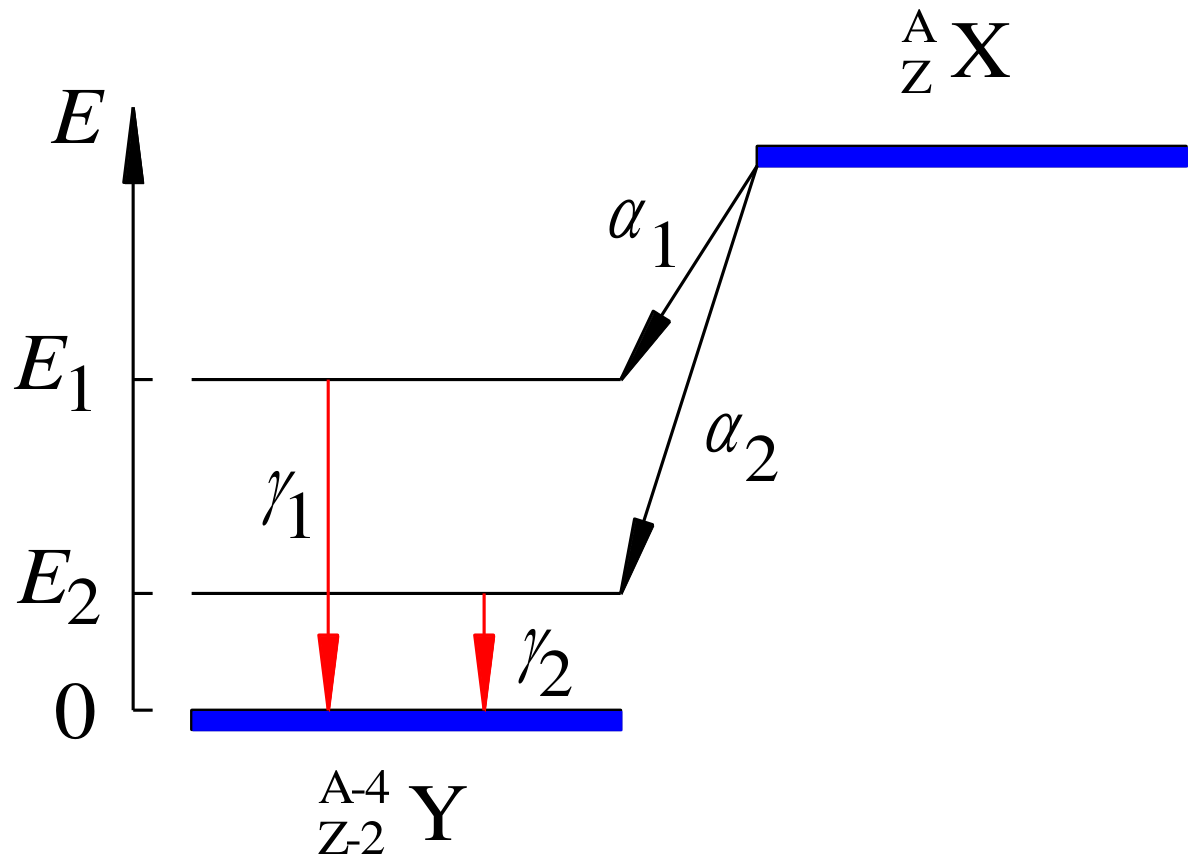
\includegraphics[width=0.3\linewidth]{theory/alpha-zerfall-schema}
    \caption{Schema eines $\alpha$-Zerfalls des Kerns X. In diesem Beispiel gibt
    es zwei $\alpha$-Zerfallskanäle, bei denen die $\alpha$-Teilchen $\alpha_1$
    oder $\alpha_2$ emittiert werden und bei denen zwei unterschiedliche 
    Energieniveaus $E_1$ und $E_2$ des Tochterkerns Y bevölkert werden. Der 
    Übergang von den Energieniveaus $E_1$ und $E_2$ in den Grundzustand von Y, 
    der per Definition die Energie 0 hat, erfolgt in diesem Beispiel unter 
    Emission der Gammaquanten $\gamma_1$ bzw. $\gamma_2$. Die energetischen 
    Grundzustände der Kerne sind blau gezeichnet --- \textsc{Quelle:} \cite[S. 30, Abb. 1]{script}}
    \label{fig:Schema Alpha-Zerfall}
\end{figure}

$\alpha$- und $\gamma$-Strahlung haben hierbei diskrete Energien, die für den
$\alpha$-Zerfall im Bereich \qty{4}{\mega\electronvolt} bis 
\qty{9}{\mega\electronvolt} und für die $\gamma$-Quanten liegen die Energien
im Bereich von \qty{10}{\kilo\electronvolt} bis \qty{3}{\mega\electronvolt}.

\subsection{\texorpdfstring{$\beta$}{Beta}-Zerfall}
$\beta$-Zerfall kommt in den drei Arten
\begin{itemize}[noitemsep, nosep]
    \item $\beta^-$-Zerfall
    \item $\beta^+$-Zerfall
    \item Elektroneneinfang
\end{itemize}
vor. In den durchgeführten Versuchen ist jedoch nur der $\beta^-$-Zerfall 
betrachtet, welcher bei Atomkernen jeder Massenzahl stattfinden kann. Die
Voraussetzung für den $\beta^-$-Zerfall ist, dass der Mutterkern X durch den
Zerfall in einen energetisch niedrigeren, stabileren Zustand des Tochterkerns
übergehen kann.
\begin{equation*}
    \isotope[A][Z]{X}_N \to \isotope[A][Z+1]{Y}_{N-1} + \beta^- + \mathbf{\bar{v}}
\end{equation*}
Auch hierbei können $\gamma$-Quanten emittiert werden, wenn beim Zerfall nicht
der Grundzustand des Tochterkerns bevölkert wird, sondern ein angeregter Zustand
bevölkert wird (vgl. \cref{fig:Schema Beta-Zerfall}). Da bei dem Zerfall neben
dem Tochterkern ein Elektron und ein Antineutrino enstehen, die Energie
aufnehmen können, hat die $\beta$-Strahlung keine diskrete Energie, sondern hat
eine kontinuierliche Energieverteilung.

\begin{figure}[H]
    \centering
    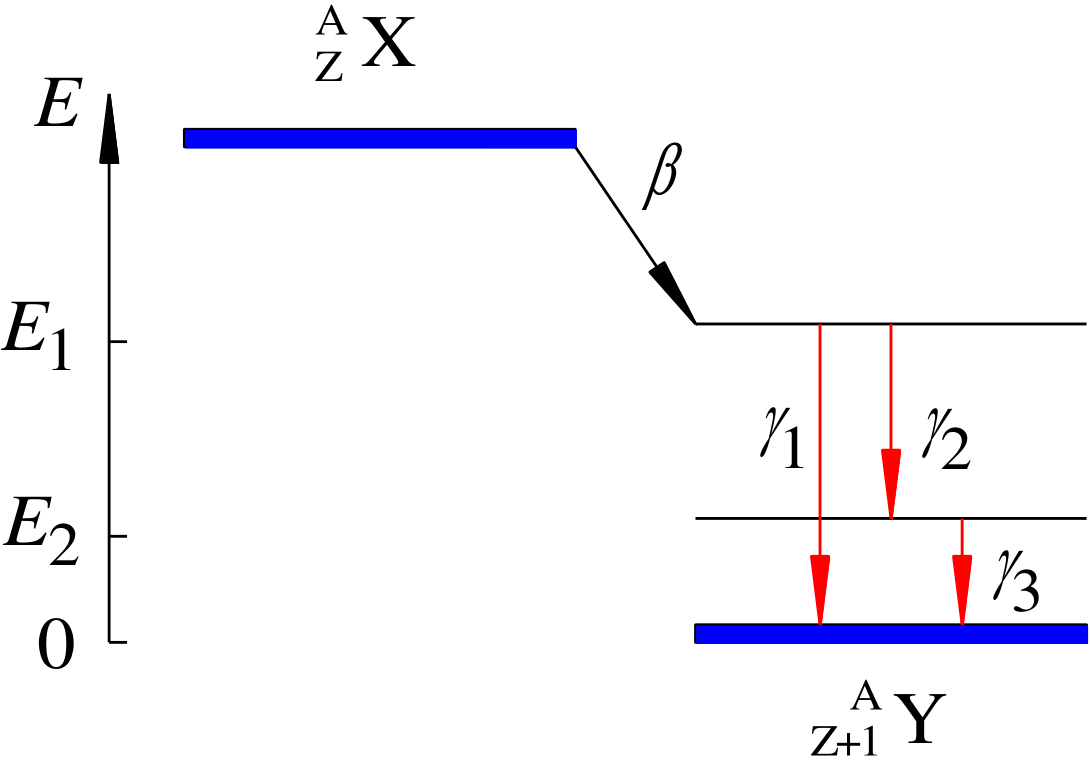
\includegraphics[width=0.3\linewidth]{theory/beta-zerfall-schema}
    \caption{Schema eines $\beta^-$-Zerfalls des Kerns X. In diesem Beispiel 
    gibt es nur einen $\beta$-Zerfallskanal, über den das Energieniveau E1 des 
    Tochterkerns Y bevölkert wird. Der Übergang von diesem Energieniveau in den 
    Grundzustand von Y kann direkt unter Emission des Gammaquants $\gamma_1$
    erfolgen, oder über den Umweg des Energieniveaus E2 unter
    Emission der Gammaquanten $\gamma_2$ und $\gamma_3$. --- 
    \textsc{Quelle:} \cite[S. 31, Abb. 2]{script}}
    \label{fig:Schema Beta-Zerfall}
\end{figure}

\section{Zerfallsgesetz und Aktivität}
Für einen eizigen Atomkern eines radioaktiven Isotops kann keine Aussage
getroffen werden, ob dieser innerhalb eines bestimmten Zeitraums zerfallen wird.
Daher können nur Aussagen über eine große Menge von Atomkernen getroffen werden.

Zu einem Zeitpunkt $t$ seien $N(t)$ Kerne eines radioaktiven Isotops X 
vorhanden. Die Zahl der innerhalb des Zeitintervalls $\mathrm{d}t$ zerfallenden
Kerne, $\mathrm{d}N(t)$ ist proportional zu $N(t)$ und $\mathrm{d}t$. Mit der
Zerfallskonstanten $\lambda$ gilt:
\begin{equation}\label{eq:Theorie - Zerfallsgleichung}
    \mathrm{d}N(t) = - \lambda \cdot N(t) \cdot \mathrm{d}t
\end{equation}
wobei das Minuszeichen die Abnahme der vorhandenen Kerne signalisiert.

Aus \cref{eq:Theorie - Zerfallsgleichung} kann abgelesen werden, dass die
Zerfallskonstante den Bruchteil der Kerne eines radioaktiven Isotops angibt, der
im Mittel pro Sekunde zerfällt.
\begin{equation}\label{eq:Zerfallskonstante}
    \lambda = \left| - \dfrac{\mathrm{d}N(t)}{N(t) \mathrm{d}t} \right|
\end{equation}

Wird nun $N_0$ definiert als die vorhandenen Atomkerne des Isotops X zum 
Zeitpunkt $t=0$, so folgt nach der Integration von 
\cref{eq:Theorie - Zerfallsgleichung} für die Zahl der nicht zefallenen Kerne
des Isotops X zum Zeitpunkt $t$ folgende Gleichung:
\begin{equation}\label{eq:Vorhandene Kerne}
    N(t) = N_0 \exp(-\lambda \cdot t)
\end{equation}

Als \textsl{Aktivität} $A$ wird die folgende Größe bezeichnet:
\begin{equation}\label{eq:Aktivität}
    A(t) = N(t) \cdot \lambda = \left| \diff{N(t)}{t} \right| = \lambda N_0 \exp(- \lambda t)
\end{equation}
Die SI-Einheit der Aktivität ist das \textsc{Becquerel}: $\qty{1}{\becquerel} = 1 \frac{\text{Zerfall}}{\unit{\second}}$
\newpage


\section{Wechselwirkung von \texorpdfstring{$\gamma$}{Gamma}-Strahlung mit Materie}
Die beim Zerfall von Isotopen freigesetze $\gamma$-Strahlung hat eine
Wechselwirkung auf Materie, welche über die folgenden drei Effekte erfolgt:
\begin{itemize}[noitemsep,nosep]
    \item innerer Fotoeffekt
    \item \textsc{Compton}-Effekt
    \item Paarbildungseffekt
\end{itemize}

In den hier beschriebenen Versuchen spielt der Paarbildungseffekt aufgrund der
Energie der verwendeten $\gamma$-Strahlung jedoch keine Rolle.

\subsection{Photoeffekt}
Unter dem inneren Photoeffekt versteht man die Totalabsorption eines
$\gamma$-Quants an der Elektronenhülle eines Atomkerns. Aufgrund der 
Impulserhaltung findet der Wechselwirkungsprozess an stark gebundenen Elektronen
statt. Das Elektron erhält hierbei die kinetische Energie $E_k$, die der
Differenz der Energie des $\gamma$-Quants ($h \cdot f$) und der Bindungsenergie
des Elektron $E_b$ enspricht:
\begin{equation}\label{eq:Kinetische Energie Photoeffekt}
    E_k = h \cdot f - E_b
\end{equation}

Die Impulserhaltung ist hierbei erfüllt, da der Atomkern einen Rückstoßimpuls
aufnimmt, wegen seiner großen Masse im Vergleich zum Elektron jedoch keine
kinetische Energie aufnimmt. Gleiches gilt für die in 
\cref{fig:Schmea Photoeffekt} gezeichnete Situation.

\begin{figure}[H]
    \centering
    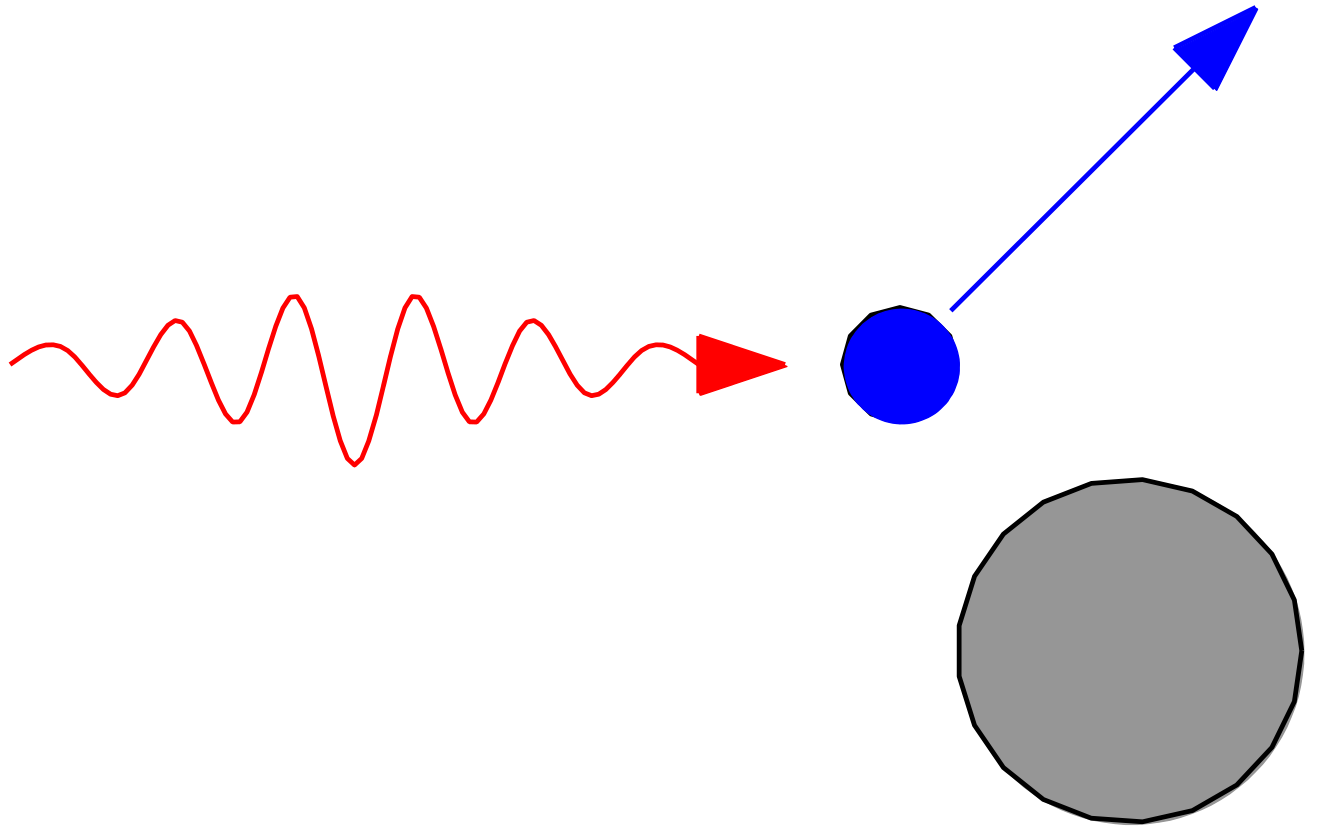
\includegraphics[width=0.3\linewidth]{theory/schema-photoeffekt}
    \caption{Prinzip des Photoeffekts. Ein $\gamma$-Quant (rot) trifft auf ein 
    Elektron (blau), das stark an den Atomkern (grau) gebunden ist. Das Elektron
     verlässt das Atom in Richtung des blauen Pfeils. --- 
     \textsc{Quelle}: \cite[S.32, Abb. 3]{script}}
    \label{fig:Schema Photoeffekt}
\end{figure}

\subsection{\textsc{Compton}-Effekt}
Die elastische und inkohärente Streuung von $\gamma$-Quanten an freien oder sehr
schwach gebundenen Elektronen heißt \textsc{Compton}-Streuung 
(vgl. \cref{fig:Schema Compton-Effekt}). Hierbei ist die vom Elektron
aufgenommene kinetische Energie $E_k$ die Differenz zwischen der Energie des
einfallenden $\gamma$-Quants ($h \cdot f$) und der Energie des gestreuten
Quants ($h \cdot f_s$):
\begin{equation}\label{eq:Kinetische Energie Compton}
    E_k = hf - hf_s
\end{equation}

\begin{figure}[H]
    \centering
    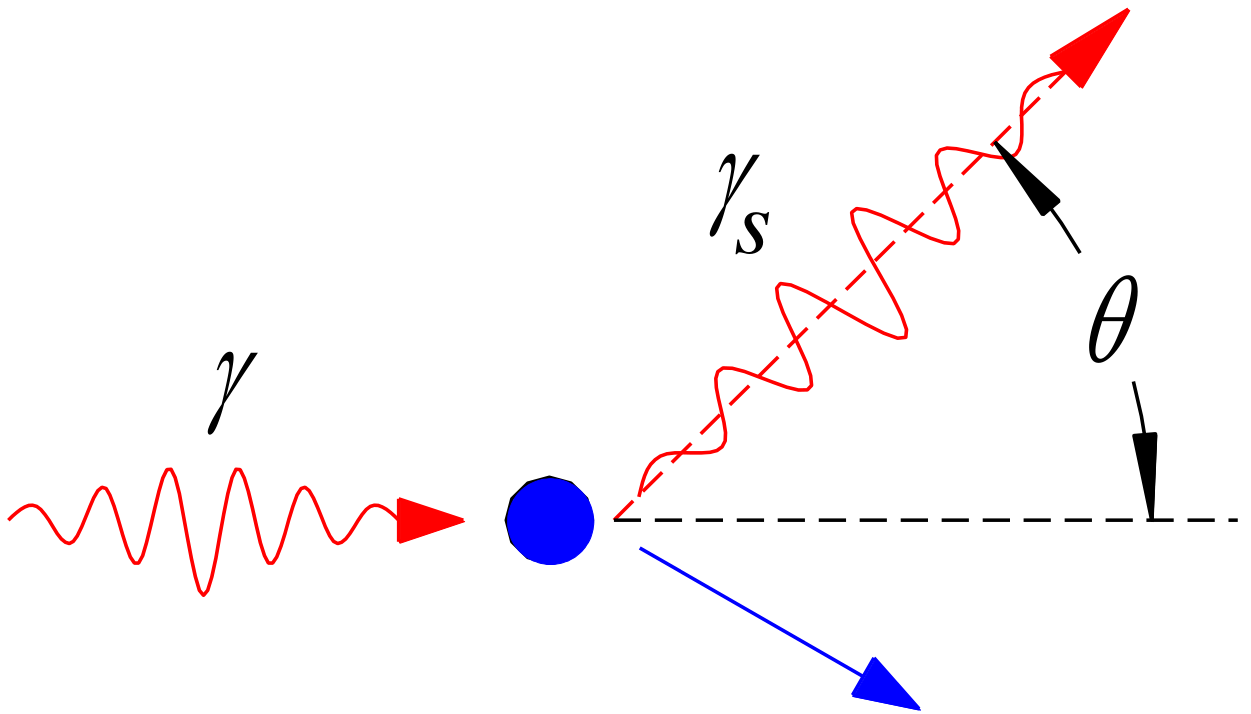
\includegraphics[width=0.3\linewidth]{theory/schema-compton}
    \caption{
        Prinzip des COMPTON-Effektes. Ein $\gamma$-Quant ($\gamma$, rot) trifft auf ein freies
        oder nur sehr schwach an einen Kern gebundenes Elektron (blau), an dem 
        es gestreut wird. Das gestreute Quant ($\gamma_s$) fliegt unter dem Winkel
        $\theta$ weiter, das Elektron in Richtung des blauen Pfeils.
    }
    \label{fig:Schema Compton-Effekt}
\end{figure}

\section{Abschwächungsgesetz}
Wird nach \cref{fig:absorbtion-dicke} der Durchgang monoenergetischer 
$\gamma$-Strahlung durch einen Absorber der Dicke $x$, mit der Intensität $I$
der Strahlung vor dem Absorber als $I_0$, so gilt für Strahlung die ohne
Wechselwirkungsprozess den Absorber verlässt:
\begin{equation}
    I(x) = I_0 \exp(-\mu x) = I_0 \exp(- (\mu_\tau + \mu_\sigma) x)
\end{equation}
wobei $\mu$ der totale lineare Abschwächungskoeffizient ist. Dieser setzt sich
aus dem linearen Abschwächungskoeffizienten für den Photoeffekt $\mu_\tau$ und
dem linearer Abschwächungskoeffizienten für den \textsc{Compton}-Effekt 
$\mu_\sigma$ zusammen.

\begin{figure}[H]
    \centering
    \begin{subfigure}[t]{0.45\linewidth}
        \centering
        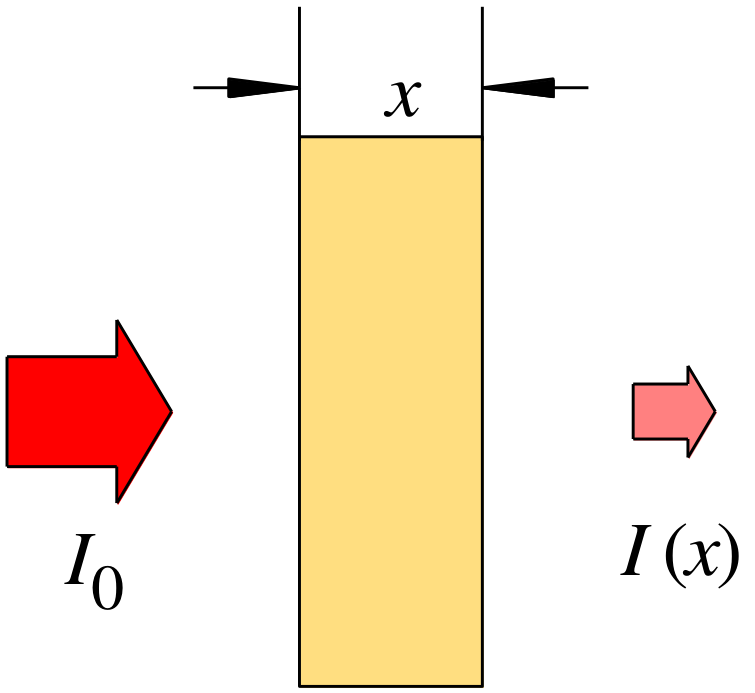
\includegraphics[width=0.5\linewidth]{theory/abschwaechung-absorber}
        \caption{
            Zur Abschwächung der Intensität $I$ einer Strahlung beim 
            Durchgang durch einen Absorber (gelb) der Dicke $x$ ---
            \textsc{Quelle}: \cite[S. 33, Abb. 5 (links)]{script}
        }
        \label{fig:absorbtion-dicke}
    \end{subfigure}
    \hfill
    \begin{subfigure}[t]{0.45\linewidth}
        \centering
        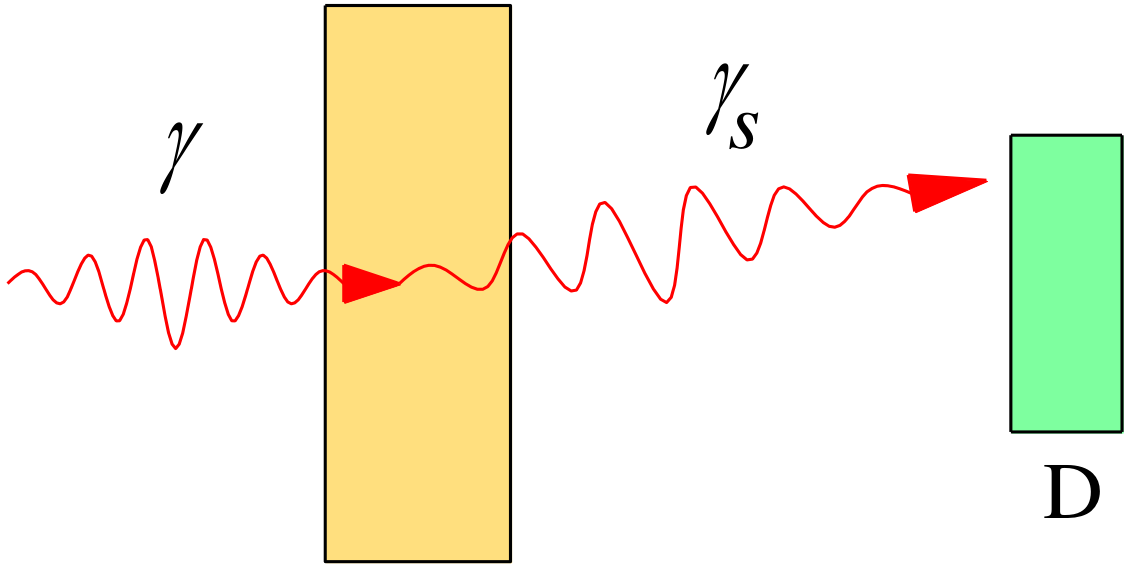
\includegraphics[width=\linewidth]{theory/abschwaechung-compton}
        \caption{
            Beispiel für ein $\gamma$-Quant, das in einem Absorber unter einem 
            kleinen Winkel \textsc{Compton}-gestreut wird. Das gestreute Quant $\gamma_s$
            verlässt den Absorber und kann bei kleinem Streuwinkel in einem 
            dahinter stehenden Detektor D nachgewiesen werden ---
            \textsc{Quelle}: \cite[S. 33, Abb. 5 (rechts)]{script}
        }
        \label{fig:absorbtion-compton}
    \end{subfigure}
    \caption{Darstellung von verschiedenen Abschwächungen}
    \label{fig:absorbtion}
\end{figure}
\end{document}